\documentclass[12pt,a4paper]{article}
\usepackage[utf8]{inputenc}
\usepackage[T1]{fontenc}
\usepackage[francais]{babel}
\usepackage{amsmath}
\usepackage{amsfonts}
\usepackage{amssymb}
\usepackage{graphicx}
\usepackage[top=2.00cm]{geometry}
\usepackage{titlesec}
%%modif des titres de section diminuer la taille
\renewcommand{\thesection}{\Roman{section}}
\titleformat{\section}
{\normalfont\bfseries\Large\scshape}{\thesection}{1em}{}
\titleformat{\subsection}
{\normalfont\bfseries\large}{\thesubsection}{1em}{}

\makeatletter
\def\@maketitle{
	
	\begin{center}
		% NoLogo
		% \vspace*{+2cm}
		
		% Corner Logo
		% \begin{flushright}
		%  
\includegraphics[width=40mm]{logo_corner}\\[4ex]
		% \end{flushright}
		
		% Top Logo
		
\includegraphics[scale=0.3]{res/logo_top}
		
		
		{\LARGE \@title }\\[4ex]
		{\large \@author}\\[4ex]
		{\large \@date}\\[8ex]
		\rule{\linewidth}{0.4pt}
	\end{center}
}
\makeatletter

\author{CHARNAY Valentin, FINOT Sylvain}
\title{Compte rendu de TP :\\[4pt] \scshape Transformateur}

\date{\today}
\begin{document}
	\maketitle
	\section*{Étude des tensions}
	\begin{center}
		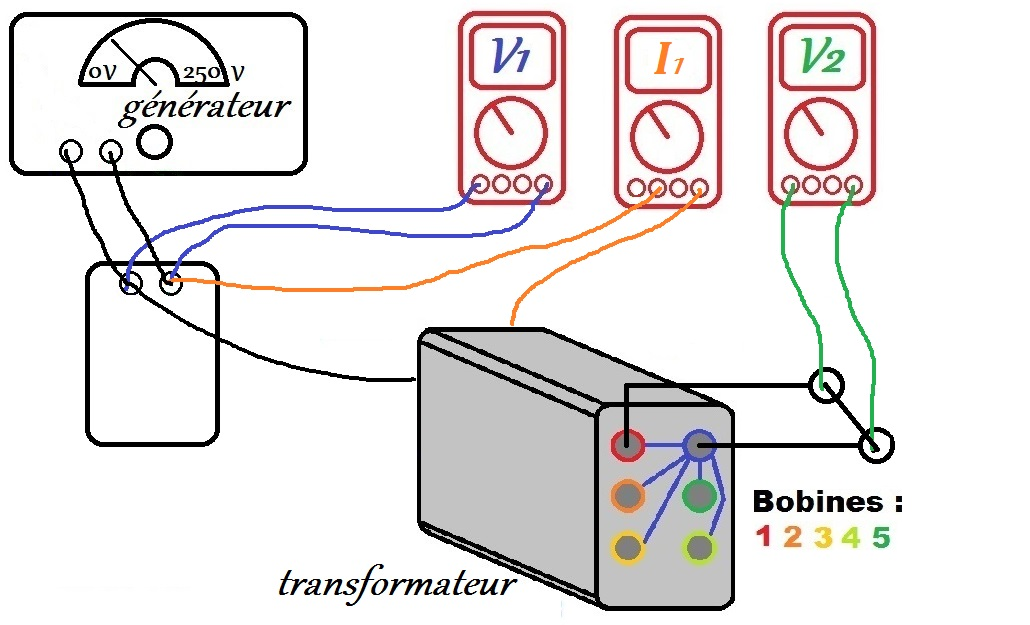
\includegraphics[scale=0.6]{schema2}
	\end{center}
	Nous avons réalisé le montage ci-dessus avec un transformateur composé de plusieurs bobinages (voir schéma du montage).
	
	Afin de gagner en temps et pouvoir directement comparer la différence entre les différents circuits, nous avons fixé $V_1$ et changé de bobine à chaque fois.
	
	On obtient alors les graphiques tiré de se tableau : 
	\begin{center}
		
		
		\begin{tabular}{cccccc}
			$V_1$ & $V_2$ de la bobine n$^{\circ}$1 & 2 & 3 & 4 & 5 \\
			\hline
			0,51  & 0,00160  & 0,02 & 0,05 & 0,07 & 0,04\\
			10,57 & 0,10019  & 0,59 & 0,99 & 0,79 & 0,28\\
			20,44 & 0,19691  & 1,17 & 1,96 & 1,57 & 0,57\\
			30,25 & 0,29305  & 1,74 & 2,93 & 2,34 & 0,86\\
			40,38 & 0,39232  & 2,34 & 3,92 & 3,13 & 1,16\\
			50,2  & 0,48856  & 2,92 & 4,89 & 3,91 & 1,45\\
		\end{tabular}
	\end{center}
	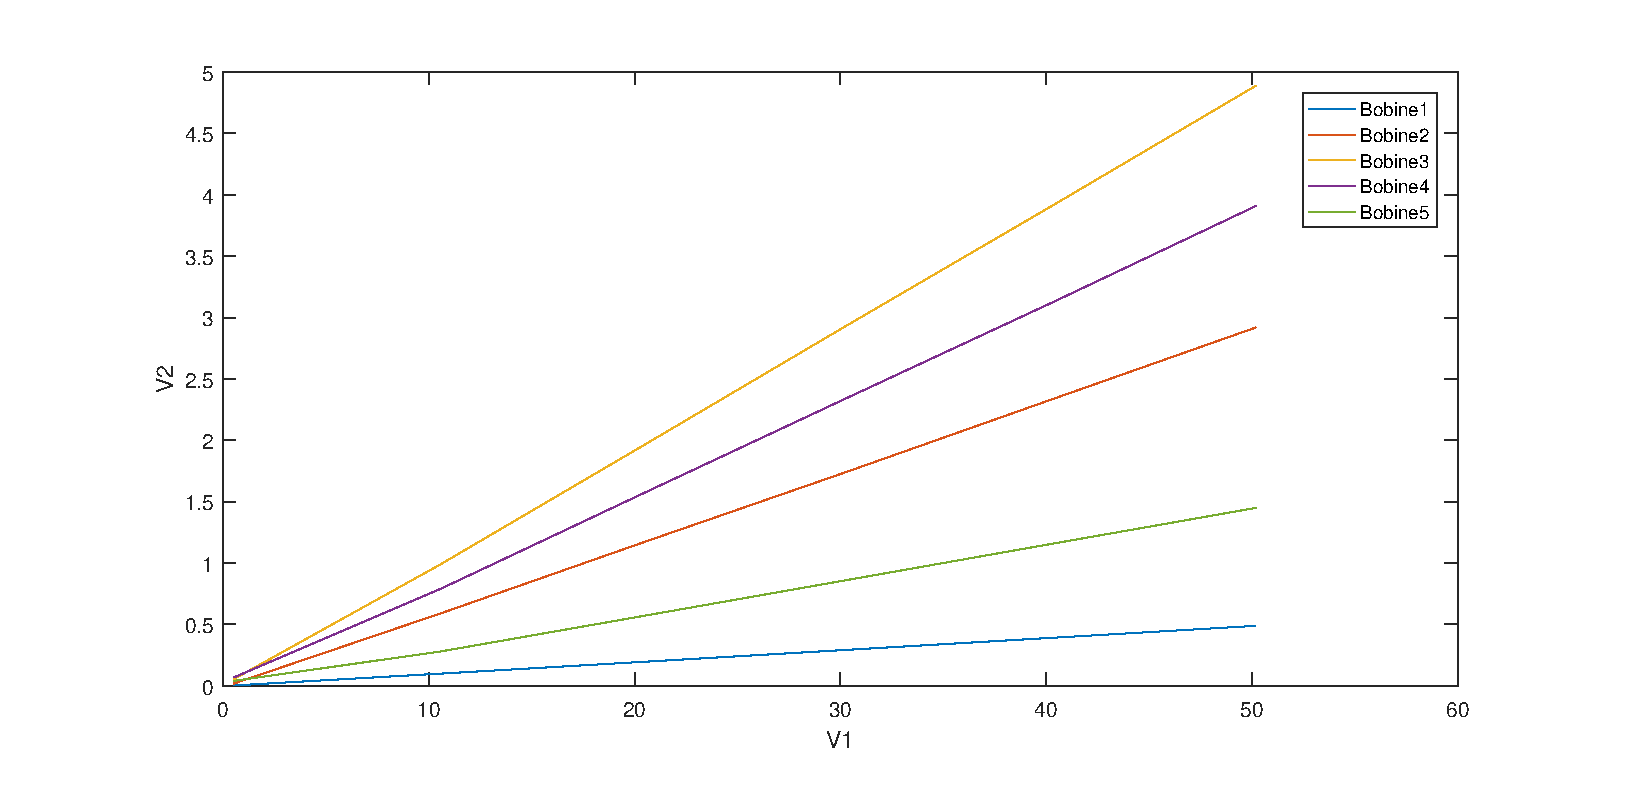
\includegraphics[width=\linewidth]{res/Bobines.eps}
	
	\bgroup
	\setlength{\tabcolsep}{1em}
	\def\arraystretch{1.25}
	\begin{tabular}{cl}
		Bobine n$^\circ$ & Equations\\
		\hline
		
		1 & $V_2=9,8.10^{-3}V_1-3,4.10^{-3}$\\
		2 & $V_2=5,85.10^{-2}V_1-2,2.10^{-2}$\\
		3 & $V_2=9,76.10^{-2}V_1-2,1.10^{-2}$\\
		4 & $V_2=7,8.10^{-2}V_1-3,7.10^{-3}$\\
		5 & $V_2=2,87.10^{-3}V_1-2,1.10^{-3}$\\
	\end{tabular}
	\egroup
	Avec m le coefficient devant $V_1$\\
	
	Le coefficient m mis en évidence dans le tableau ci-dessus correspond au rapport du transformateur $\frac{n_1}{n_2}$ montre la différence d'efficacité du bobinage en fonction du nombre de spire de celle-ci (la taille du bobinage n'est pas directement corrélé au numéro de la bobine).
	
	\pagebreak
	\section*{Étude du courant}
	\begin{center}
		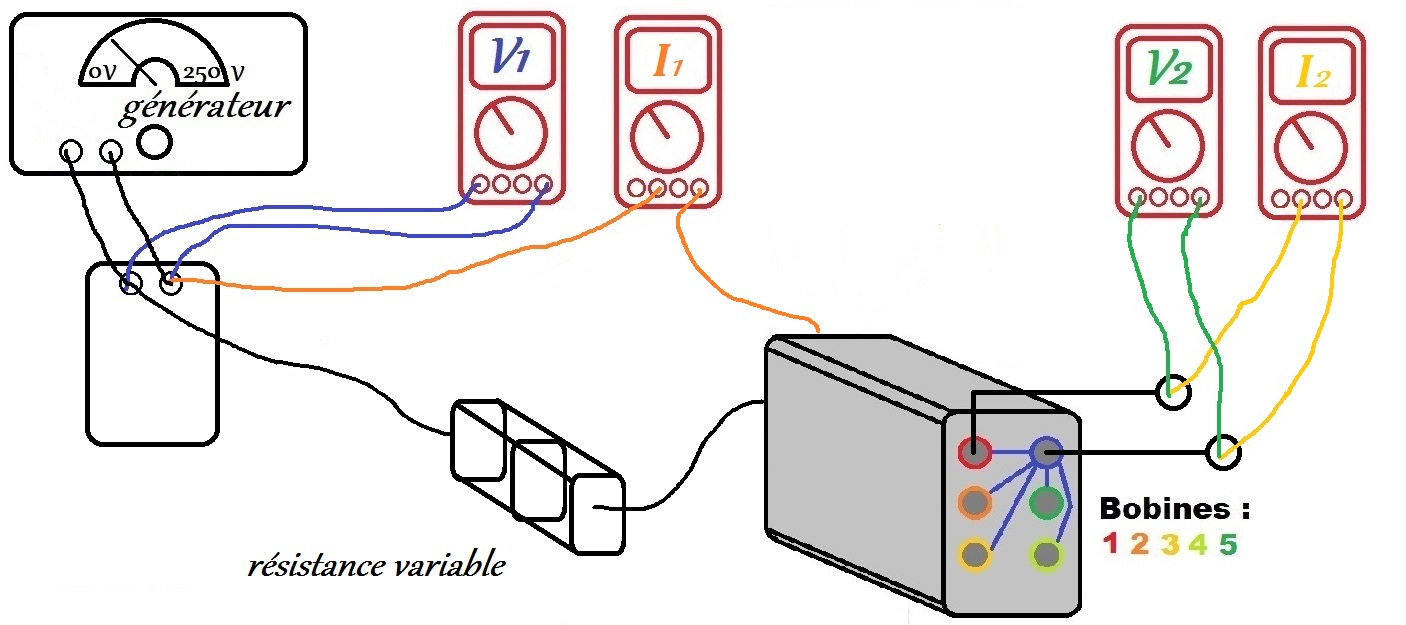
\includegraphics[scale=0.6]{schema1}
	\end{center}
	\begin{itemize}
		\item[$\circ$]
		En mesurant la puissance à vide $P_0$ du montage en branchant un wattmètre en parallèle avec $V_1$ on peut alors déterminer les coefficients $R_f$ et $L_f$ qui caractérise les pertes d'hystérésis du transformateur.
		$$R_f = \dfrac{V_{1}^2}{P_0} \hspace{1cm} L_f = \dfrac{V_{1}^2}{\sqrt{V_{1}^2 I_{1}^2 - P_{0}^2}}$$
		
		En effectuant plusieurs mesures, on obtient :
		$$R_f \approx \dfrac{28.77^2}{0.58} \approx 1427\hspace{0.2cm} \Omega \hspace{0.5cm} et \hspace{0.5cm}
		R_f \approx \dfrac{45.38^2}{1.33} \approx 1542\hspace{0.2cm} \Omega$$
		
		
		\item[$\circ$]
		Nous avons branché un oscilloscope en entrée (signal $V_1$) et en sortie de la résistance variable ($I_1$ grâce à la chute de tension) afin de voir le décalage entre les deux : plus $V_1$ est grand plus le signal modélisant $I_1$ est déformé.
		
		On obtient alors un signal décalé de 7,6 ms soit un déphasage de : \\
		10,5ms $\rightarrow$ $\pi$ \\
		7,6ms $\rightarrow \dfrac{7,6\pi}{10,5} \approx\dfrac{5\pi}{7}$
		\pagebreak
		\item[$\circ$]
		Dans le montage ci-dessus, on étudiera la variation de courant de sortie $I_2$ en fonction de $I_1$ que l'on fait varier à la l'œil avec la résistance variable.
		
		On obtient alors le diagramme suivant, le rapport $\dfrac{I_1}{I_2}$  en fonction de $I_2$:
		\begin{center}
			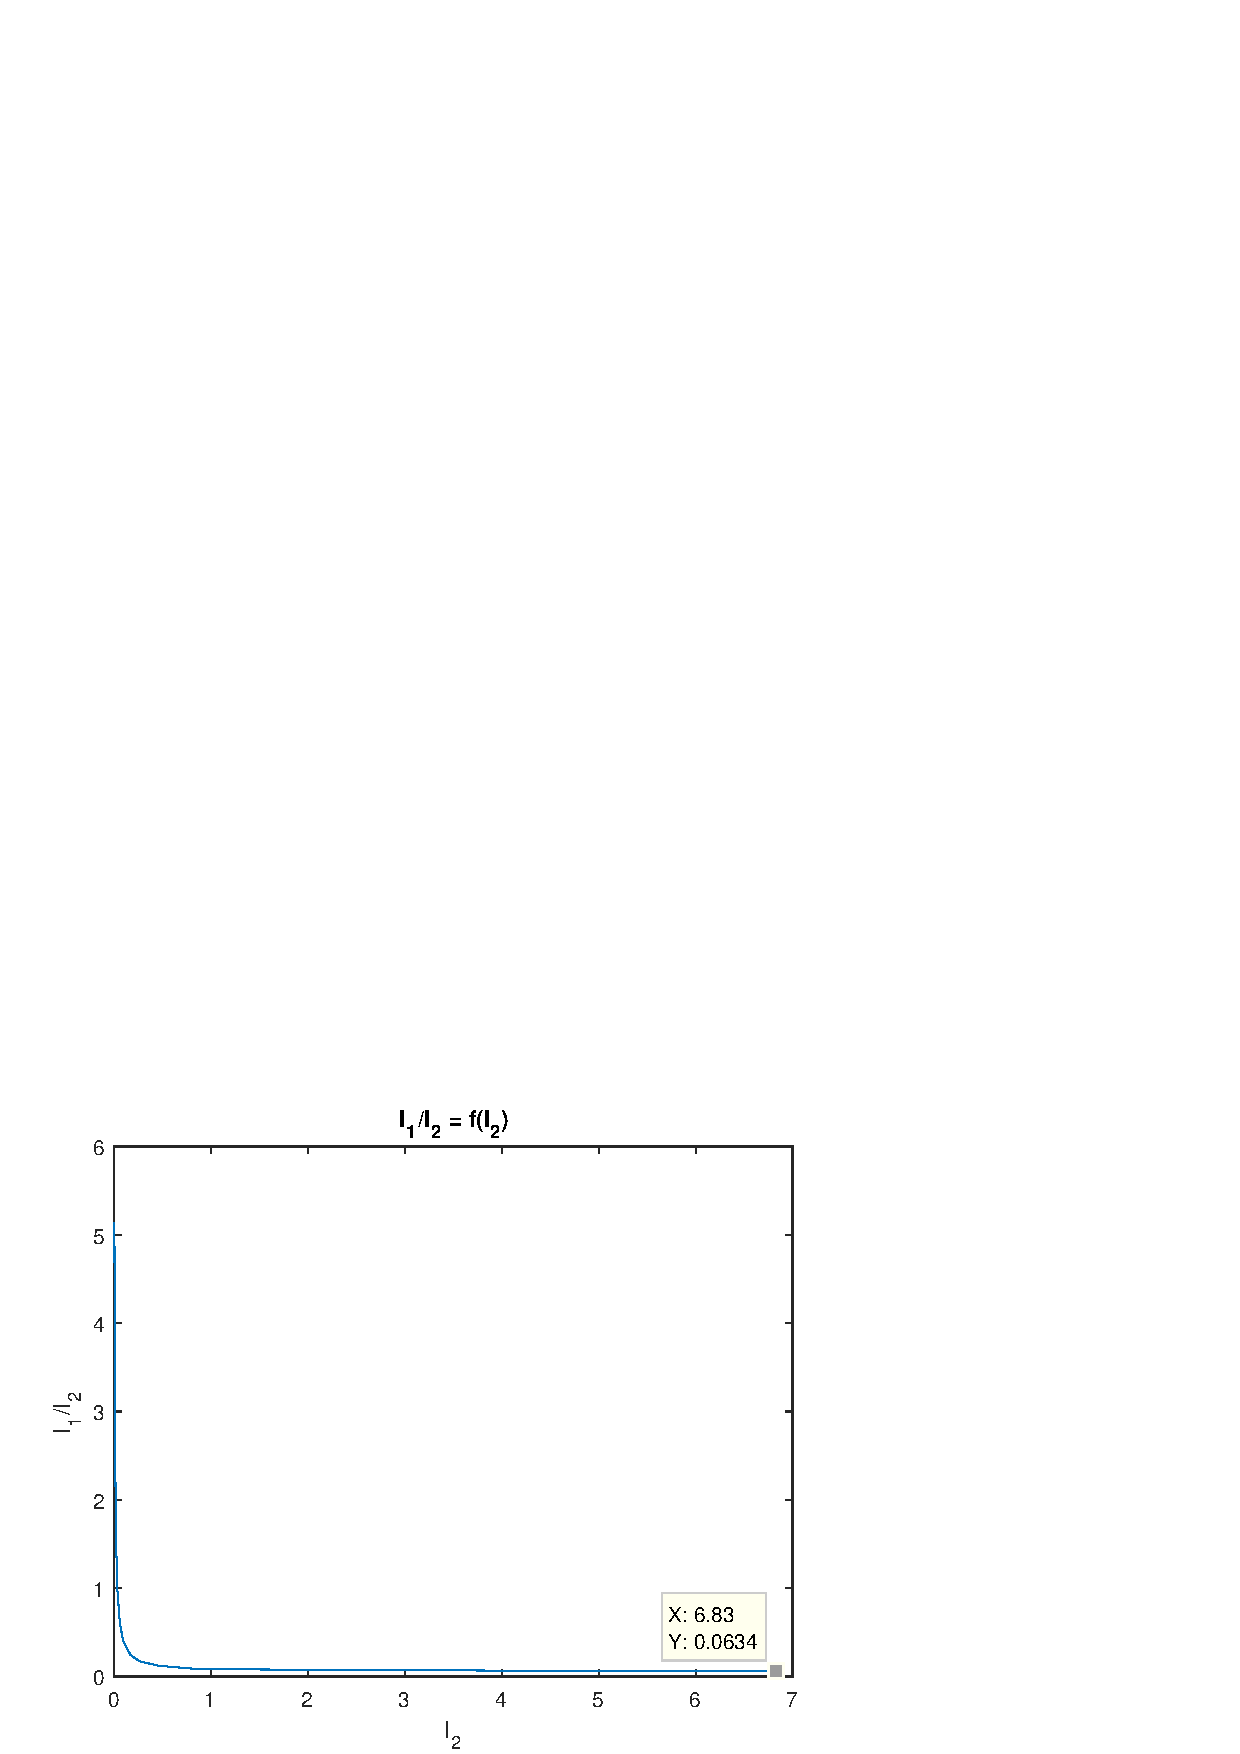
\includegraphics[width=0.8\linewidth]{res/I1I2}
		\end{center}
		
		
		On remarque alors que la courbe semble être modélisée par une exponentielle décroissante tendant vers la valeur $1/16$.
		On peut comparer cette limite à la valeur de m déterminée dans la première partie :
		$$m_2=5,85.10^{-2}\approx1/17$$ 
		
		Un autre point important que l'on remarque en traçant $\dfrac{V_2}{V_1} =f(I_2)$, le rapport n'est pas constant et est décroissant. Cela signifie que lorsque la sortie nécessite plus de courant, la tension chute et n'est plus égale à la tension à vide.\\
		\begin{center}
			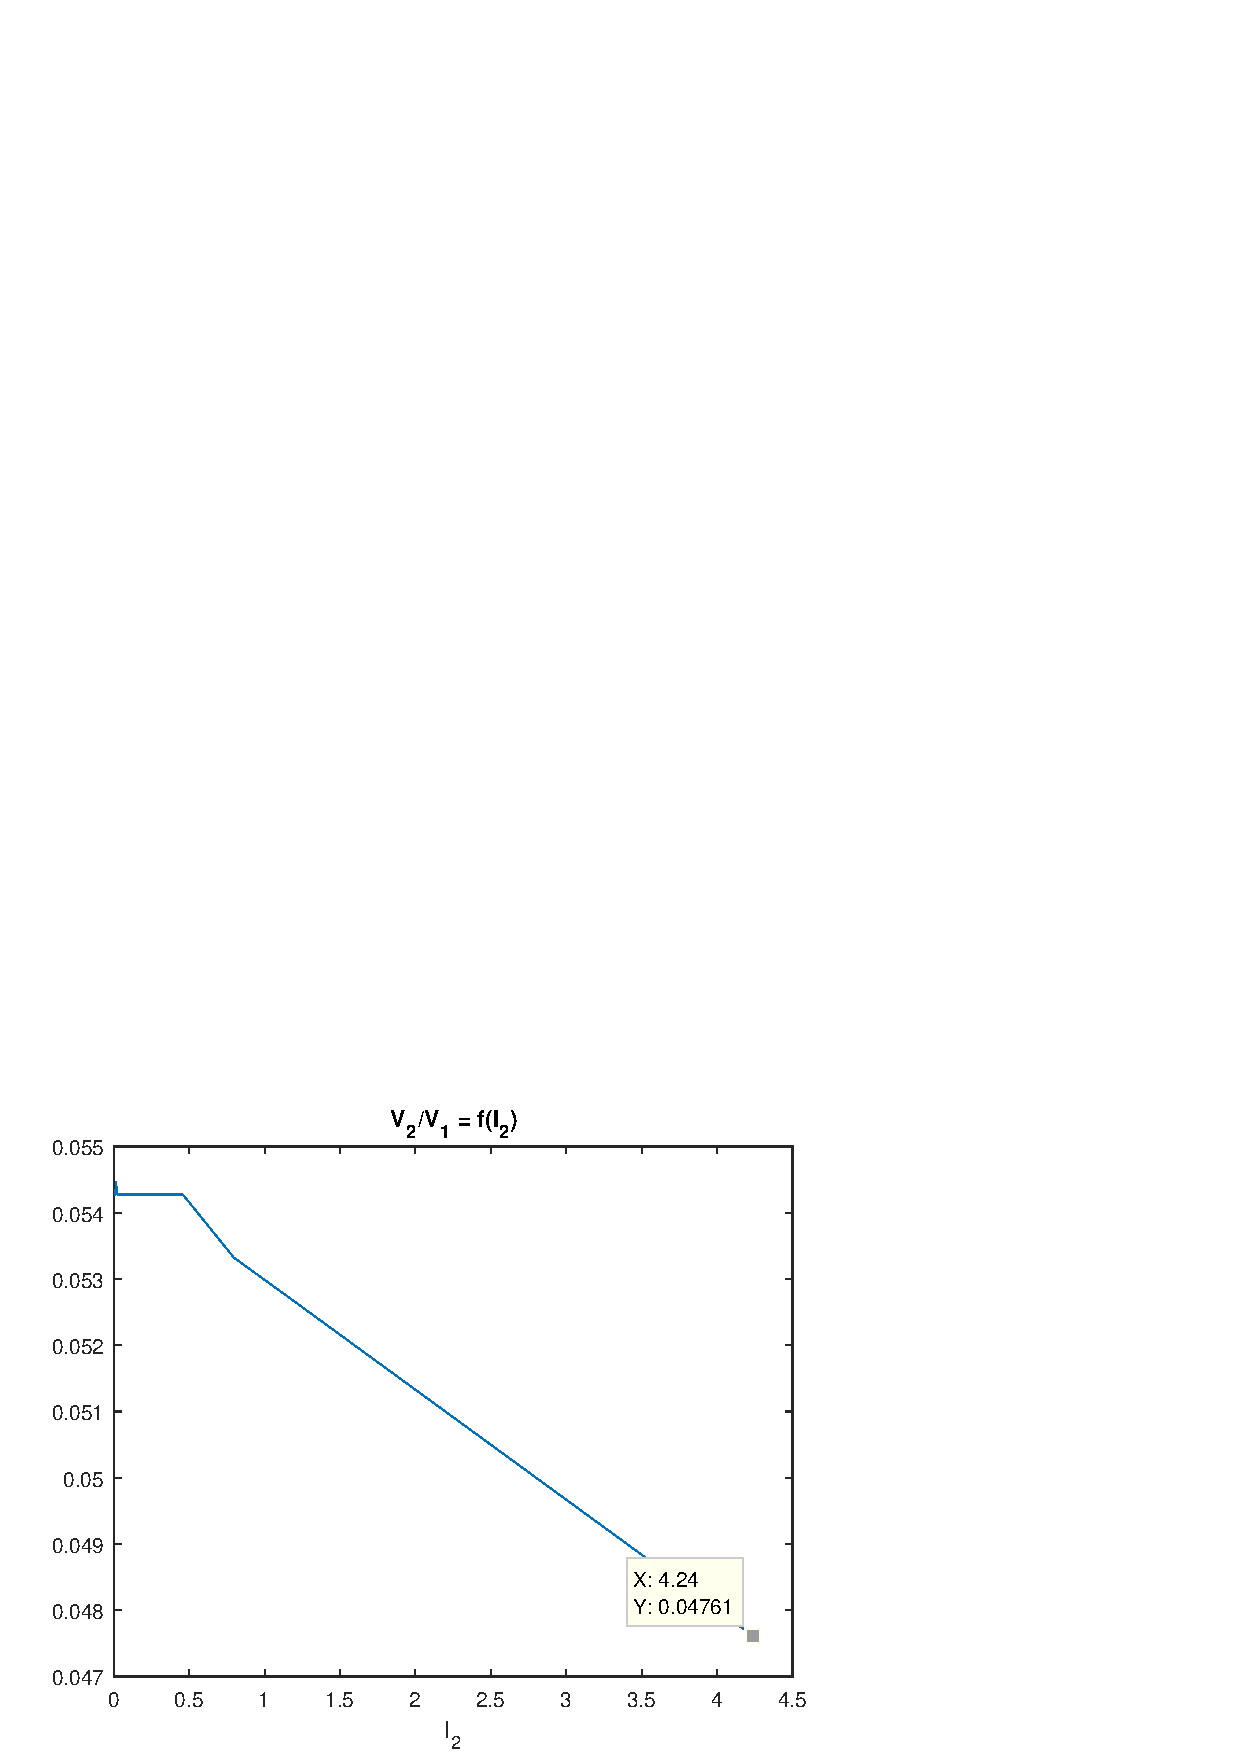
\includegraphics[width=0.8\linewidth]{res/chutetension}
		\end{center} 
	\end{itemize}
\end{document}

